\documentclass[11pt]{article}

% ---------- Packages ----------
\usepackage[a4paper,margin=2.2cm]{geometry}
\usepackage{amsmath,amssymb,amsthm,mathtools}
\usepackage{physics}
\usepackage{siunitx}
\sisetup{per-mode=symbol}
\usepackage{booktabs}
\usepackage{array}
\usepackage{enumitem}
\usepackage{tikz}
\usetikzlibrary{arrows.meta,calc,positioning,decorations.pathmorphing,patterns,shapes.geometric,decorations.markings}
\usepackage{tcolorbox}
\usepackage{capt-of}
\usepackage{hyperref}
\hypersetup{colorlinks=true,linkcolor=blue!50!black,citecolor=blue!50!black,urlcolor=blue!50!black}
\usepackage{xcolor}
\usepackage{fancyhdr}
\usepackage{titlesec}
\usepackage{caption}
\captionsetup{font=small,labelfont=bf}

% ---------- Colours ----------
\definecolor{defcol}{RGB}{235,245,255}
\definecolor{defbar}{RGB}{60,110,180}
\definecolor{intcol}{RGB}{255,247,225}
\definecolor{intbar}{RGB}{200,140,20}
\definecolor{keycol}{RGB}{235,255,240}
\definecolor{keybar}{RGB}{40,140,80}
\definecolor{exccol}{RGB}{250,235,240}
\definecolor{excbar}{RGB}{170,50,90}

% ---------- Boxes ----------
\newtcolorbox{defbox}[1][]{colback=defcol,colframe=defbar,boxrule=0.6pt,arc=1pt,
left=6pt,right=6pt,top=4pt,bottom=4pt,title={#1},fonttitle=\bfseries,
coltitle=black, colbacktitle=defcol, boxsep=1pt,before skip=8pt,after skip=8pt}
\newtcolorbox{intuition}[1][Intuition]{colback=intcol,colframe=intbar,boxrule=0.6pt,arc=1pt,
left=6pt,right=6pt,top=4pt,bottom=4pt,title={#1},fonttitle=\bfseries,
coltitle=black,colbacktitle=intcol,boxsep=1pt,before skip=8pt,after skip=8pt}
\newtcolorbox{keyresult}[1][Key Result]{colback=keycol,colframe=keybar,boxrule=0.7pt,arc=1pt,
left=6pt,right=6pt,top=4pt,bottom=4pt,title={#1},fonttitle=\bfseries,
coltitle=black,colbacktitle=keycol,boxsep=1pt,before skip=8pt,after skip=8pt}
\newtcolorbox{worked}[1][Worked Example]{colback=exccol,colframe=excbar,boxrule=0.6pt,arc=1pt,
left=6pt,right=6pt,top=4pt,bottom=4pt,title={#1},fonttitle=\bfseries,
coltitle=black,colbacktitle=exccol,boxsep=1pt,before skip=8pt,after skip=8pt}

% ---------- Headers ----------
\pagestyle{fancy}
\fancyhf{}
\renewcommand{\headrulewidth}{0.4pt}
\lhead{\small\textit{Atmospheric Thermodynamics \& Radiative Balance}}
\rhead{\small\thepage}

\titleformat{\section}{\large\bfseries\color{defbar}}{\thesection}{0.6em}{}
\titleformat{\subsection}{\normalsize\bfseries\color{black}}{\thesubsection}{0.6em}{}

\newcommand{\ddz}[1]{\dfrac{d#1}{dz}}
\newcommand{\pdz}[1]{\dfrac{\partial #1}{\partial z}}
\newcommand{\Rd}{R_d}
\newcommand{\Rv}{R_v}
\newcommand{\Rstar}{R^{*}}

\title{\vspace{-1.5cm}\textbf{Atmospheric Thermodynamics, Hydrostatics,\\ Forces, and Radiative Balance}\\[4pt]
\large Consolidated Lecture Notes}
\author{}
\date{}

\begin{document}
\maketitle
\thispagestyle{fancy}
\vspace{-1.2cm}

\begin{abstract}
\noindent These notes consolidate and extend material from six source documents covering: the ideal gas law and its application to moist air (virtual temperature), the hydrostatic equation and geopotential, atmospheric composition and mixing ratios, the fundamental forces governing atmospheric motion (pressure gradient force), and the global radiative energy balance including greenhouse models and radiative--convective equilibrium. The treatment is derivation-first: every relation used later is either derived here or explicitly flagged as an empirical input. A glossary of notation precedes the physical content.
\end{abstract}

\tableofcontents
\newpage

% =====================================================================
\section*{Notation and Terminology Key}
\addcontentsline{toc}{section}{Notation and Terminology Key}

\begin{defbox}[Conventions used throughout]
\begin{itemize}[leftmargin=1.4em]
\item \textbf{System vs.\ parcel}: An \emph{air parcel} is a small, identifiable blob of air treated as a thermodynamic system (fixed mass unless stated otherwise). \emph{Eulerian} description = fields $T(x,y,z,t)$ etc.\ at fixed points in space; \emph{Lagrangian} description = properties of a parcel followed as it moves. This distinction matters because ``the temperature is changing'' can mean either (a) at a fixed point, air of different origin is arriving, or (b) a given parcel is itself heating/cooling.
\item \textbf{Intensive vs.\ extensive}: quantities per unit mass (specific volume $\alpha=1/\rho$, specific heat, specific gas constant $R$) are \emph{specific} (intensive); quantities like total volume $V$, total internal energy $U$ are extensive.
\item \textbf{Subscripts}: $d$ = dry air, $v$ = water vapour, $s$ = surface, $e$ = emission (top-of-atmosphere equivalent blackbody), $a$ = atmosphere (in slab radiative models), $0$ = reference/sea level.
\item $p$ = pressure (Pa or hPa; $1\ \text{hPa}=100\ \text{Pa}$), $T$ = absolute temperature (K), $\rho$ = density (\si{\kg\per\cubic\m}), $\alpha=1/\rho$ = specific volume (\si{\cubic\m\per\kg}).
\item $R^{*}=8.3145\ \si{\joule\per\mol\per\kelvin}$: \emph{universal} gas constant (same for all gases, per mole). $R = R^{*}/M$: \emph{specific} gas constant for a particular gas of molar mass $M$ (per unit \emph{mass}).
\item $N_A = 6.022\times10^{23}\ \si{\per\mol}$: Avogadro's number. $k = R^{*}/N_A = 1.381\times10^{-23}\ \si{\joule\per\kelvin}$: Boltzmann's constant (gas constant \emph{per molecule}).
\item Geopotential $\Phi$, geopotential height $Z=\Phi/g_0$, scale height $H$.
\item Radiative balance: $S_0$ = solar constant, $\alpha_p$ = planetary albedo, $T_e$ = emission temperature, $T_s$ = surface temperature, $\sigma=5.67\times10^{-8}\ \si{\watt\per\square\m\per\kelvin\tothe{4}}$ = Stefan--Boltzmann constant, $\epsilon$ = atmospheric IR absorptivity/emissivity.
\item ``Isothermal'' = constant temperature; ``isobaric'' = constant pressure; ``adiabatic'' = no heat exchange ($dq=0$); these are used conceptually below (e.g.\ the dry adiabatic lapse rate in \S\ref{sec:radconv}) but their full first-law-of-thermodynamics derivation is not part of the source excerpts and is flagged where used.
\item A vertical bar/overline, e.g.\ $\overline{T_v}$, denotes a \emph{pressure-weighted layer mean} (defined precisely in \S\ref{sec:hypsometric}), not a time average.
\end{itemize}
\end{defbox}

\noindent\textbf{Prerequisite knowledge assumed} (standard 12th-grade physics/chemistry, \emph{not} re-derived): Boyle's law, Charles' laws, the mole concept, Newton's laws of motion and gravitation, basic calculus (partial derivatives, definite integrals), Taylor expansion to first order, and the Stefan--Boltzmann / Wien laws as empirical facts of blackbody radiation (their statistical-mechanical derivation is out of scope, but their use is fully derived here).

\newpage
% =====================================================================
\section{The Ideal Gas Law: From Molecules to Moist Air}

\subsection{The equation of state}

For $m$ kg of a gas occupying volume $V$ at pressure $p$ and absolute temperature $T$,
\begin{equation}
pV = mRT, \qquad \text{or equivalently} \qquad p = \rho R T, \qquad p\alpha = RT
\label{eq:idealgas}
\end{equation}
where $\rho = m/V$ is density, $\alpha = 1/\rho$ is specific volume, and $R$ is the \emph{specific} gas constant of that particular gas (units $\si{\joule\per\kg\per\kelvin}$). Equation \eqref{eq:idealgas} is an empirical equation of state that all atmospheric gases obey to excellent approximation over the range of pressures and temperatures found in the atmosphere.

At fixed $T$, \eqref{eq:idealgas} reduces to \textbf{Boyle's law} ($pV=\text{const}$); at fixed $p$ it gives \textbf{Charles' first law} ($V\propto T$); at fixed $V$ it gives \textbf{Charles' second law} ($p\propto T$). These three empirical gas laws are simply special cases of \eqref{eq:idealgas} obtained by holding one variable fixed.

\begin{intuition}[Kinetic theory picture]
Model a gas as $N$ identical elastic particles of mass $m_0$ bouncing randomly inside a container (Wallace \& Hobbs' ``handball court'' analogy). Pressure arises from momentum transfer to the walls: each collision transfers momentum $\propto m_0 v$, and the collision \emph{frequency} on a wall is also $\propto v$ (faster molecules arrive more often) and $\propto 1/V$ (larger box $\Rightarrow$ fewer wall encounters per unit time, at fixed number density this is really a statement about geometry). Hence:
\begin{itemize}[leftmargin=1.4em]
\item Increase $V$ at fixed $v$ (fixed $T$): collision frequency $\propto 1/V$, so pressure $\propto 1/V$ — recovers Boyle's law.
\item Increase $v$ at fixed $V$: both the momentum \emph{per} collision and the collision \emph{frequency} scale as $v$, so pressure $\propto v^2 \propto$ mean kinetic energy $\propto T$ — recovers Charles' second law (kinetic theory identifies temperature with mean molecular kinetic energy).
\end{itemize}
This is a mnemonic, not a substitute for the statistical-mechanical derivation of \eqref{eq:idealgas}, which is taken here as an empirical input matching experiment.
\end{intuition}

\subsection{Moles, Avogadro's number, and the universal gas constant}

Define a \textbf{mole} of a substance as its molecular weight $M$ expressed in grams. The number of moles in mass $m$ (grams) is
\begin{equation}
n = \frac{m}{M}.
\end{equation}
\textbf{Avogadro's hypothesis}: equal volumes of any gas at the same $p,T$ contain equal numbers of molecules. Equivalently, $1$ mol of \emph{any} substance contains the same number of molecules, $N_A = 6.022\times10^{23}\,\text{mol}^{-1}$ (Avogadro's number). A direct consequence: if you take the \emph{same number of moles} of any two gases, the constant relating $pV$ to $nT$ is identical for both — this defines the \textbf{universal gas constant}
\begin{equation}
pV = R^{*}T \quad (\text{1 mol}), \qquad pV = nR^{*}T \quad (n \text{ mol}), \qquad R^{*}=8.3145\ \si{\joule\per\mol\per\kelvin}.
\label{eq:universal}
\end{equation}
Because $R^{*}$ is universal but $R$ (per unit \emph{mass}) is gas-specific, comparing \eqref{eq:idealgas} (for 1 kg, $m=1$) with \eqref{eq:universal} written for $M$ grams ($=10^{-3}M$ kg, i.e.\ 1 mole) of the gas:
\begin{equation}
\boxed{R = \frac{R^{*}}{M}}
\end{equation}
with $M$ in kg/mol; if instead $M$ is quoted in g/mol (as is conventional, e.g.\ $M_d=28.97$ g/mol below), insert a factor of $1000$ as in \eqref{eq:Rd}.

The gas constant \emph{per molecule} (rather than per unit mass or per mole) is \textbf{Boltzmann's constant}:
\begin{equation}
k = \frac{R^{*}}{N_A} = 1.381\times10^{-23}\ \si{\joule\per\kelvin}, \qquad\text{so that}\qquad p = n_0 k T,
\label{eq:boltzmann}
\end{equation}
where $n_0$ is the number density (molecules per unit volume). Equation \eqref{eq:boltzmann} is the ``per-molecule'' form of the ideal gas law and is the most fundamental of the three forms \eqref{eq:idealgas}, \eqref{eq:universal}, \eqref{eq:boltzmann} — the other two follow from it by multiplying by $N_A$ (moles) or by the total molecule count (mass).

\subsection{The gas constant for dry air}
\label{sec:Rd}

Dry air is a \emph{mixture} of gases (see \S\ref{sec:composition} for composition). Define the \textbf{apparent molecular weight} of a mixture as the total mass of all constituents divided by the total number of moles:
\begin{equation}
M_d = \frac{\sum_i m_i}{\sum_i m_i/M_i}.
\label{eq:apparentM}
\end{equation}
\emph{Derivation of why this is the right averaging}: from \eqref{eq:universal}, each constituent gas $i$, if it alone occupied the mixture's volume at the mixture's $T$, would satisfy $p_i' V = n_i R^* T$ with $n_i = m_i/M_i$. Summing over species (using Dalton's law below) and requiring the mixture to obey $pV = \left(\sum m_i\right) R_{\text{mix}} T$ with a single effective $R_{\text{mix}} = R^*/M_d$ forces \eqref{eq:apparentM}.

For dry air, $M_d = 28.97\ \si{\g\per\mol}$ (i.e., $28.97\times10^{-3}\ \si{\kg\per\mol}$), so
\begin{equation}
\Rd = \frac{1000\,R^{*}}{M_d} = \frac{1000\times 8.3145}{28.97} = 287.0\ \si{\joule\per\kg\per\kelvin}.
\label{eq:Rd}
\end{equation}
(The factor $1000$ converts $M_d$ in g/mol to give $\Rd$ per \emph{kg}, since $R^*$ is defined per mole = per $M_d$ grams.) Then for dry air,
\begin{equation}
p_d \alpha_d = \Rd T
\label{eq:idealgasdry}
\end{equation}
where $p_d,\alpha_d$ are the partial pressure and specific volume of the dry-air component.

Similarly for water vapour, molecular weight $M_w = 18.016\ \si{\g\per\mol}$:
\begin{equation}
\Rv = \frac{1000 R^{*}}{M_w} = \frac{1000\times8.3145}{18.016} = 461.51\ \si{\joule\per\kg\per\kelvin}, \qquad e\,\alpha_v = \Rv T,
\label{eq:Rv}
\end{equation}
where $e$ is the partial pressure of water vapour (vapour pressure) and $\alpha_v$ its specific volume. Note $\Rv > \Rd$ because $M_w < M_d$ (water vapour molecules are lighter, so fewer grams make up a mole, so the ``constant per unit mass'' is larger).

Define the useful ratio
\begin{equation}
\varepsilon \equiv \frac{\Rd}{\Rv} = \frac{M_w}{M_d} = 0.622.
\label{eq:epsilon}
\end{equation}

\subsection{Dalton's law of partial pressures}
Dalton's law: the total pressure of a mixture of non-reacting gases equals the sum of the \textbf{partial pressures}, where the partial pressure of species $i$ is the pressure it \emph{would} exert at the mixture's temperature if it alone occupied the entire volume:
\begin{equation}
p = \sum_i p_i.
\label{eq:dalton}
\end{equation}
For moist air (dry air + water vapour only, to good approximation): $p = p_d + e$.

\begin{worked}[Total pressure of a dry-air/water-vapour mixture]
At $T=273\ \text{K}$, suppose the partial density of dry air alone is $\rho_d=1.275\ \si{\kg\per\cubic\m}$ and of water vapour alone $\rho_v = 4.770\times10^{-3}\ \si{\kg\per\cubic\m}$. Find total pressure.

\textbf{Solution.} Apply \eqref{eq:idealgasdry}-type relations directly in density form, $p_i = \rho_i R_i T$:
\[
p_d = \rho_d \Rd T = (1.275)(287.0)(273.2) = 9.997\times10^{4}\ \text{Pa} = 999.7\ \text{hPa}
\]
\[
e = \rho_v \Rv T = (4.770\times10^{-3})(461.51)(273.2) = 601.4\ \text{Pa} = 6.014\ \text{hPa}
\]
By Dalton's law \eqref{eq:dalton}, $p = p_d + e = 999.7+6.014 = 1005.7 \approx 1006\ \text{hPa}$.
\end{worked}

\subsection{Virtual temperature}
\label{sec:virtualT}

\textbf{Motivation.} Moist air is a mixture with a smaller apparent molecular weight than dry air (water vapour is ``light''), so by \eqref{eq:Rd}-type reasoning its effective gas constant $R_{\text{moist}} > \Rd$ and depends on how much vapour is present — inconvenient, since humidity is highly variable. The standard trick: keep using $\Rd$ always, but replace the real temperature $T$ with a fictitious \textbf{virtual temperature} $T_v \ge T$ that absorbs the humidity dependence.

\textbf{Derivation.} Consider volume $V$ of moist air, total mass $= m_d + m_v$ (dry air mass + vapour mass), at pressure $p$, temperature $T$. Density:
\begin{equation}
\rho = \frac{m_d+m_v}{V} = \rho_d' + \rho_v'
\end{equation}
where $\rho_d' = m_d/V$ and $\rho_v'=m_v/V$ are \textbf{partial densities} (i.e., each constituent's mass divided by the \emph{total} volume $V$ — not the volume it would occupy alone). Apply the ideal gas law \eqref{eq:idealgas} in the form $p=\rho RT$ separately to each constituent, using their \emph{partial pressures} $p_d'$ (dry air) and $e$ (vapour), each of which acts over the full volume $V$ at temperature $T$:
\begin{equation}
p_d' = \rho_d' \Rd T, \qquad e = \rho_v' \Rv T.
\end{equation}
By Dalton's law $p = p_d' + e$. Solve each relation for the partial density and substitute into $\rho = \rho_d'+\rho_v'$:
\begin{equation}
\rho = \frac{p-e}{\Rd T} + \frac{e}{\Rv T} = \frac{p}{\Rd T}\left[1 - \frac{e}{p}\left(1-\frac{\Rd}{\Rv}\right)\right] = \frac{p}{\Rd T}\left[1-\frac{e}{p}(1-\varepsilon)\right].
\end{equation}
Rearranged into ideal-gas form $p=\rho \Rd T_v$:
\begin{equation}
\boxed{p = \rho \Rd T_v}, \qquad
\boxed{T_v \equiv \dfrac{T}{1-\dfrac{e}{p}(1-\varepsilon)}}
\label{eq:Tv}
\end{equation}
with $\varepsilon = 0.622$ from \eqref{eq:epsilon}. Since $0<\varepsilon<1$, the denominator is $<1$, so $T_v > T$ always: \textbf{virtual temperature is always greater than or equal to actual temperature}, and equals it only for completely dry air ($e=0$).

\begin{defbox}[Physical meaning of $T_v$]
$T_v$ is \emph{the temperature dry air would need to have in order to possess the same density as the actual moist air, at the same pressure}. Because moist air is less dense than dry air at equal $p,T$ (replacing heavier N$_2$/O$_2$ molecules with lighter H$_2$O reduces mass per mole), moist air must be ``pretend-heated'' to $T_v>T$ to make a dry-air computation reproduce its (lower) density. In practice $T_v-T$ is only a few kelvin even in very warm, humid air, since $e/p$ rarely exceeds a few percent.
\end{defbox}

% =====================================================================
\section{Atmospheric Composition}
\label{sec:composition}

\subsection{Composition of dry air}
Dry air is $\sim$99\% N$_2$ (78.08\%) and O$_2$ (20.95\%) by volume, with Ar (0.93\%), and trace ($<0.1\%$ combined) but radiatively/chemically crucial species: CO$_2$, O$_3$, CH$_4$, N$_2$O, CO, and water vapour (highly variable, up to $\sim$3\% by volume near the surface in the tropics).

\begin{table}[h!]
\centering
\small
\begin{tabular}{@{}lcp{4.3cm}p{4.3cm}@{}}
\toprule
Constituent & Mixing ratio & Vertical profile & Controlling process \\
\midrule
N$_2$ & 78.08\% & well-mixed & inert, vertical mixing \\
O$_2$ & 20.95\% & well-mixed & inert, vertical mixing \\
Ar & 0.93\% & well-mixed & inert, vertical mixing \\
H$_2$O$^*$ & $\le 3\%$ & falls sharply with height in troposphere & evaporation/condensation, transport \\
CO$_2^*$ & $\sim$380 ppmv & well-mixed & surface + anthropogenic sources \\
O$_3^*$ & $\sim$10 ppmv (strat.) & peaks in stratosphere & photochemical production/destruction \\
CH$_4^*$ & 1.8 ppmv & well-mixed in troposphere, falls above & surface production, OH oxidation \\
N$_2$O$^*$ & 320 ppbv & well-mixed in troposphere, falls above & surface/anthropogenic, photolysis \\
\bottomrule
\end{tabular}
\caption{Approximate tropospheric composition of air. $^*$ = radiatively active (``greenhouse'') gas. ppmv/ppbv = parts per million/billion \emph{by volume}, i.e. by mole fraction.}
\end{table}

\begin{intuition}[Why trace gases matter despite tiny abundance]
N$_2$ and O$_2$ are diatomic and (to good approximation) do not absorb/emit efficiently in the infrared: a diatomic molecule's only internal motions are a single vibrational mode and rotations about axes with negligible moment of inertia change, giving very weak dipole-moment fluctuations. \emph{Triatomic} molecules (H$_2$O, CO$_2$, O$_3$) have multiple vibrational and rotational modes with bending motions that strongly change the molecular dipole moment, making them efficient IR absorbers/emitters. Hence composition (mass fraction) and radiative importance are almost inversely correlated: the 1\%-abundance triatomics dominate the planet's infrared energy budget (\S\ref{sec:absorption}).
\end{intuition}

\subsection{Measures of relative abundance}
Let subscript $d$ denote dry air (used as reference mass since it is materially conserved for a parcel, unlike total moist-air mass, which changes on condensation).

\begin{align}
\textbf{Mass mixing ratio:}\quad & r_i = \frac{m_i}{m_d} \quad \text{(dimensionless; g/kg for water vapour, ppmm for trace gases)}\\
\textbf{Molar fraction:}\quad & N_i = \frac{n_i}{n} = \frac{p_i}{p} = \frac{V_i}{V} \quad \text{(from dividing \eqref{eq:idealgasdry}-type relations)} \\
\textbf{Number density:}\quad & [i] = \frac{N_A}{M_i}\rho_i
\end{align}
For a trace species (mass negligible compared to dry air), $N_i \approx r_i/\varepsilon_i$ where $\varepsilon_i = M_i/M_d$ (compare \eqref{eq:epsilon} for water vapour specifically).

\begin{defbox}[Why mixing ratio, not absolute concentration?]
Absolute concentration ($\rho_i$ or $n_0$) changes when a parcel simply \emph{expands or contracts} (compressibility), even if no molecules of species $i$ are created or destroyed. The mass mixing ratio $r_i=m_i/m_d$ uses the \emph{dry-air mass in the same parcel} as reference, and $m_d$ is fixed for an individual parcel (no diffusion assumed) — so $r_i$ changes only through genuine sources/sinks (condensation, chemistry), not through volume changes. A quantity that is constant for a parcel absent such sources/sinks is called \textbf{conserved}, and conserved quantities are ideal \emph{tracers} of air motion.
\end{defbox}

\subsection{Equation of state for a mixture (general form)}
Generalizing \S\ref{sec:Rd}: for a mixture with mean specific gas constant $\overline R = \sum_i m_i R_i / m$ (mass-weighted average of the constituent specific gas constants) and mean molar mass $\overline M = R^*/\overline R$, the mixture obeys $pV = m\overline R T$, exactly analogous to a single gas. This is the general statement of which \eqref{eq:idealgasdry} (dry air) and \eqref{eq:Tv} (moist air, folded into $T_v$ instead of a variable $R$) are special cases.

% =====================================================================
\section{Hydrostatic Balance, Geopotential, and the Hypsometric Equation}
\label{sec:hydrostatic}

\subsection{Derivation of the hydrostatic equation}

Consider a vertical column of air of unit horizontal cross-sectional area. Take a thin slab between heights $z$ and $z+\delta z$, of mass $\rho\,\delta z$ (per unit area). Two vertical forces act (per unit area):
\begin{itemize}[leftmargin=1.4em]
\item \textbf{Weight (downward):} $g\rho\,\delta z$, where $g=g(z)$ is local gravitational acceleration.
\item \textbf{Net pressure force (upward):} pressure on the lower face exceeds that on the upper face since $p$ decreases with height. If the pressure change across the slab is $\delta p$ (a \emph{negative} number, since $p$ decreases upward), the net upward force per unit area is $-\delta p$.
\end{itemize}
\textbf{Hydrostatic balance} is the statement that these two forces balance (no net vertical acceleration):
\begin{equation}
-\delta p = g\rho\,\delta z \quad\Longrightarrow\quad \lim_{\delta z\to 0}\ \frac{\partial p}{\partial z} = -g\rho.
\label{eq:hydrostatic}
\end{equation}
This is the \textbf{hydrostatic equation}. The negative sign guarantees $p$ decreases with height. Equivalently, using $\rho=1/\alpha$,
\begin{equation}
\frac{\partial p}{\partial z} = -\frac{g}{\alpha}, \qquad\text{or}\qquad g\,dz = -\alpha\,dp.
\label{eq:hydrostatic2}
\end{equation}

\begin{intuition}
This is exactly the ``stack of mattresses'' picture: the pressure at any level equals the weight (per unit area) of everything stacked above it. It is an excellent approximation for large-scale atmospheric motion (horizontal scales $\gg$ vertical scale) because the true vertical acceleration is 2--3 orders of magnitude smaller than either term in \eqref{eq:hydrostatic} individually — the atmosphere is never far from exact hydrostatic balance except in intense convection.
\end{intuition}

\textbf{Total pressure at height $z$}: integrate \eqref{eq:hydrostatic} from $z$ to $\infty$ (using $p(\infty)=0$):
\begin{equation}
p(z) = \int_z^{\infty} g\rho\,dz'.
\label{eq:pweight}
\end{equation}
i.e.\ pressure at any level is simply the weight of the entire atmospheric column above that level, per unit area. At sea level with the real Earth's topography averaged out, this gives $p_0 \approx 1013\ \text{hPa} \equiv 1\ \text{atm}$.

\subsection{Geopotential}
Define the \textbf{geopotential} $\Phi(z)$ as the work required to raise 1 kg from sea level ($z=0$) to height $z$ against gravity:
\begin{equation}
d\Phi = g\,dz \quad\Longrightarrow\quad \Phi(z) = \int_0^z g(z')\,dz', \qquad \Phi(0)\equiv 0.
\label{eq:geopotdef}
\end{equation}
Units: $\text{J}\,\text{kg}^{-1} = \text{m}^2\text{s}^{-2}$. Using \eqref{eq:hydrostatic2}, $d\Phi = g\,dz = -\alpha\,dp$, i.e.
\begin{equation}
d\Phi = -\alpha\,dp.
\label{eq:geopotalt}
\end{equation}
This is useful because meteorological data (radiosondes) measure $p,T$, not $\rho$ or $z$ directly.

\textbf{Geopotential height} is geopotential expressed in length units, using a globally averaged \emph{constant} reference gravity $g_0 = 9.81\ \si{\meter\per\second\squared}$:
\begin{equation}
Z \equiv \frac{\Phi(z)}{g_0} = \frac{1}{g_0}\int_0^z g(z')\,dz'.
\label{eq:geopotheight}
\end{equation}
Since $g$ decreases very slightly with height (true gravity falls as $1/r^2$ from Earth's centre, plus centrifugal effects), $Z$ is slightly less than $z$ at a given true (geometric) height, with the difference growing at higher altitude (see table below). $Z$ is the natural vertical coordinate for energetics because it is a direct measure of gravitational potential energy per unit mass ($g_0 Z = \Phi$ exactly, by construction).

\begin{table}[h!]
\centering
\begin{tabular}{@{}cccc@{}}
\toprule
$z$ (km) & $Z$ (km) & $g$ (\si{\meter\per\second\squared}) \\
\midrule
0 & 0 & 9.81 \\
1 & 1.00 & 9.80 \\
10 & 9.99 & 9.77 \\
100 & 98.47 & 9.50 \\
500 & 463.6 & 8.43 \\
\bottomrule
\end{tabular}
\caption{Geometric height $z$ vs. geopotential height $Z$ at 40$^\circ$ latitude. Below $\sim$100 km, $Z\approx z$ to within 2\%.}
\end{table}

\subsection{Combining hydrostatic balance with the ideal gas law}

From \eqref{eq:hydrostatic2}: $dz = -\alpha\,dp/g$. Use the moist-air ideal gas law \eqref{eq:Tv}, $p\alpha = \Rd T_v$, so $\alpha = \Rd T_v/p$:
\begin{equation}
d\Phi = g\,dz = -\alpha\,dp = -\Rd T_v\,\frac{dp}{p} = -\Rd T_v\, d(\ln p).
\label{eq:geopot_dp}
\end{equation}
This is the master differential relation connecting geopotential (hence height) to pressure and (virtual) temperature. Everything in \S\ref{sec:hypsometric}--\S\ref{sec:scaleheight} below follows by integrating \eqref{eq:geopot_dp}.

\subsection{Scale height and the isothermal atmosphere}
\label{sec:scaleheight}

If $T_v$ is constant (isothermal atmosphere) with height, integrate \eqref{eq:geopot_dp} from level 1 to level 2:
\begin{equation}
\Phi_2-\Phi_1 = -\Rd T_v \ln\!\left(\frac{p_2}{p_1}\right) = \Rd T_v\ln\!\left(\frac{p_1}{p_2}\right).
\end{equation}
Dividing by $g_0$:
\begin{equation}
Z_2-Z_1 = H\ln\!\left(\frac{p_1}{p_2}\right), \qquad \boxed{H \equiv \frac{\Rd T_v}{g_0}} \quad\text{(\textbf{scale height})}.
\label{eq:scaleheight}
\end{equation}
Equivalently, solving for pressure as a function of height above a reference level $Z_1$:
\begin{equation}
p(Z) = p_1\exp\!\left[-\frac{Z-Z_1}{H}\right].
\label{eq:expdecay}
\end{equation}
$H$ is the vertical distance over which pressure falls by a factor of $1/e$. For $T_v \approx 255\ \text{K}$ (typical tropospheric/stratospheric mean), $H\approx \dfrac{287\times255}{9.81}\approx 7.5\ \text{km}$.

\begin{defbox}[Species-dependent scale height above the turbopause]
Below the \emph{turbopause} ($\sim$105 km), turbulent mixing keeps the atmosphere ``well-mixed'' — all species share the \emph{same} scale height because bulk motion, not molecular diffusion, controls transport, so \eqref{eq:scaleheight} with the mixture's $\Rd$ applies uniformly. \emph{Above} the turbopause, transport is by molecular diffusion, and each species independently satisfies barometric decay \eqref{eq:expdecay} with \emph{its own} $H_i = R^* T/(M_i g_0)$ (from \eqref{eq:idealgas} applied per species). Lighter species (e.g., H) have larger $H_i$ and therefore fall off more slowly than heavier species (e.g., O) — the atmosphere becomes compositionally stratified by mass at high altitude.
\end{defbox}

\begin{worked}[Diffusive separation above the turbopause]
Given: number density ratio $[\text{O}]/[\text{H}] = 10^5$ at $Z=200$ km; isothermal atmosphere at $T=2000$ K between 200 and 1400 km. Find the ratio at $Z=1400$ km.

\textbf{Solution.} At fixed $T$, number-density ratio = pressure ratio (ideal gas law, same $T,V$). Each species independently obeys \eqref{eq:expdecay} with its own scale height $H_i = R^*T/(M_i g_0)$:
\[
H_{\rm O} = \frac{8.3145\times2000}{16\times10^{-3}\times9.81} = 1.06\times10^{5}\ \text{m}, \qquad
H_{\rm H} = \frac{8.3145\times2000}{1\times10^{-3}\times9.81} = 1.695\times10^{6}\ \text{m}.
\]
Then
\[
\frac{[\text{O}]_{1400}}{[\text{H}]_{1400}} = \frac{[\text{O}]_{200}}{[\text{H}]_{200}}\exp\!\left[-1200\ \text{km}\left(\frac{1}{H_{\rm O}}-\frac{1}{H_{\rm H}}\right)\right] = 10^5 \exp(-10.6) \approx 2.5.
\]
Physically: over 1200 km, the heavy species (O) has decayed far more than the light species (H), collapsing the initial factor-of-$10^5$ excess of O down to a factor of only 2.5.
\end{worked}

\subsection{The hypsometric equation (general, non-isothermal case)}
\label{sec:hypsometric}

If $T_v$ varies with height, define the \textbf{pressure-weighted mean virtual temperature} between levels $p_1$ (lower) and $p_2$ (upper) as
\begin{equation}
\overline{T_v} \equiv \frac{\displaystyle\int_{p_2}^{p_1} T_v\,d(\ln p)}{\displaystyle\int_{p_2}^{p_1} d(\ln p)} = \frac{\displaystyle\int_{p_2}^{p_1}T_v\,d(\ln p)}{\ln(p_1/p_2)}.
\label{eq:Tvmean}
\end{equation}
Then integrating \eqref{eq:geopot_dp} exactly as before but pulling $\overline{T_v}$ out of the integral by definition:
\begin{equation}
\boxed{Z_2-Z_1 = \frac{\Rd \overline{T_v}}{g_0}\ln\!\left(\frac{p_1}{p_2}\right) = \overline{H}\ln\!\left(\frac{p_1}{p_2}\right)}
\label{eq:hypsometric}
\end{equation}
— the \textbf{hypsometric equation}. $Z_2-Z_1$ is called the (geopotential) \textbf{thickness} of the layer between pressure surfaces $p_1$ and $p_2$. Historically $\overline{T_v}$ was estimated graphically from a radiosonde sounding by requiring equal areas on either side of the mean-value line on a $T_v$ vs.\ $\ln p$ plot (areas $ABC=CDE$ in the classic diagram) — this is just a graphical implementation of the area-under-curve definition \eqref{eq:Tvmean}.

\begin{keyresult}[Thickness $\propto$ mean temperature]
Because \eqref{eq:hypsometric} says thickness is directly proportional to $\overline{T_v}$, a \emph{warmer} layer occupies more geometrical depth between the same two pressure surfaces than a \emph{colder} layer. This single fact underlies:
\begin{itemize}[leftmargin=1.4em]
\item Why upper-level pressure/height maps ``bulge'' upward over warm regions and sag over cold regions.
\item Why a warm-core system (e.g.\ a hurricane, warm at its centre relative to surroundings) must have its low-pressure signature (depression of isobaric surfaces) \emph{weaken with height} — thin layers above the warm core partially cancel the surface depression as one ascends.
\item Why some upper-level lows are ``cold-core'' below their level of maximum intensity and effectively ``warm-core'' above it, if they don't extend to the surface.
\end{itemize}
\end{keyresult}

\begin{worked}[Thickness of the 1000--500 hPa layer]
Compute the 1000--500 hPa thickness (a) in the tropics, $\overline{T_v}=288\ \text{K}$; (b) at the poles, $\overline{T_v}=233\ \text{K}$.

\textbf{Solution.} From \eqref{eq:hypsometric}, $\Delta Z = \dfrac{\Rd \overline{T_v}}{g_0}\ln 2 = 20.3\,\overline{T_v}\ \text{m}$ (using $\Rd=287$, $g_0=9.81$, $\ln 2 = 0.693$; check: $287\times0.693/9.81=20.3$).
\begin{align*}
(a)\ \overline{T_v}=288\ \text{K}: &\quad \Delta Z = 20.3\times288 = 5846\ \text{m} = 585\ \text{dam (decametres)}\\
(b)\ \overline{T_v}=233\ \text{K}: &\quad \Delta Z = 20.3\times233 = 4730\ \text{m} = 473\ \text{dam}
\end{align*}
The tropical (warm) column is $\sim$1100 m ``taller'' between the same two pressure surfaces than the polar (cold) column — a direct, quantitative illustration of the Key Result above.
\end{worked}

\begin{worked}[Geopotential height of the 1000 hPa surface]
Given sea-level pressure $p_0=1014$ hPa and scale height $H\approx8$ km, find $Z_{1000\,\text{hPa}}$.

\textbf{Solution.} From \eqref{eq:hypsometric} with $p_1=p_0$, $p_2=1000$ hPa, $Z_1=0$:
\[
Z_{1000} = H\ln\!\left(\frac{p_0}{1000}\right) = H\ln\!\left(1+\frac{p_0-1000}{1000}\right)\approx H\left(\frac{p_0-1000}{1000}\right)
\]
using $\ln(1+x)\approx x$ for $x\ll1$ (here $x=0.014$). With $H=8000$ m: $Z_{1000}\approx 8(p_0-1000) = 8\times14=112$ m.
This also gives the rule of thumb: \emph{near sea level, pressure falls by about 1 hPa per 8 m of ascent} (since $H\approx 8$ km and the linearized relation is $p_0-p \approx p_0 Z/H$, and $p_0\approx1000$ hPa makes the coefficient $\approx1/8\ \text{hPa/m}$).
\end{worked}

\subsection{Reduction of pressure to sea level}
For a station at elevation $Z_g$ (ground) with surface pressure $p_g$, the hypsometric equation \eqref{eq:hypsometric} applied to the layer between the ground and sea level ($Z_0=0$) gives $Z_g - 0 = \overline{H}\ln(p_0/p_g)$, so
\begin{equation}
p_0 = p_g\exp\!\left(\frac{Z_g}{\overline H}\right) = p_g \exp\!\left(\frac{g_0 Z_g}{\Rd \overline{T_v}}\right).
\label{eq:sealevelreduction}
\end{equation}
This is why weather maps report \emph{sea-level-reduced} pressure rather than raw station pressure: without the correction, every mountain station would show artificially low pressure simply due to elevation, swamping the synoptic (weather-system) signal one actually wants to see.

\subsection{Constant pressure surfaces: geometric picture}

\begin{center}
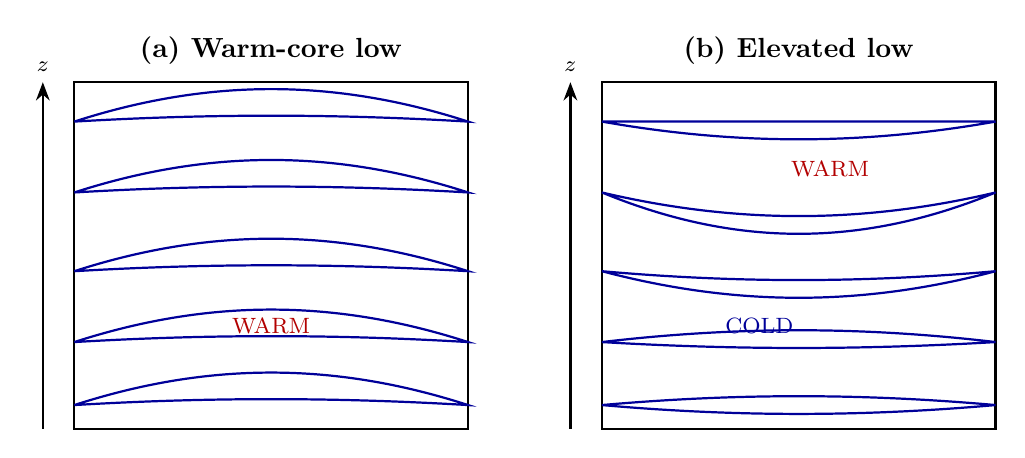
\begin{tikzpicture}[scale=1.0]
% Panel (a): warm core low
\begin{scope}
\draw[thick] (0,0) rectangle (5,4.4);
\node[above] at (2.5,4.5) {\textbf{(a) Warm-core low}};
\foreach \y/\lab in {0.3/1000, 1.1/850, 2.0/700, 3.0/500, 3.9/300} {
  \draw[thick,blue!60!black] (0,\y) .. controls (1.7,\y+0.55) and (3.3,\y+0.55) .. (5,\y)
       .. controls (3.3,\y+0.1) and (1.7,\y+0.1) .. (0,\y);
}
\node[red!70!black] at (2.5,1.3) {\footnotesize WARM};
\draw[-Stealth,thick] (-0.4,0) -- (-0.4,4.4) node[above]{\footnotesize $z$};
\end{scope}
% Panel (b): elevated cold/warm core low
\begin{scope}[xshift=6.7cm]
\draw[thick] (0,0) rectangle (5,4.4);
\node[above] at (2.5,4.5) {\textbf{(b) Elevated low}};
\foreach \y/\dir in {0.3/0, 1.1/0.05, 2.0/-0.3, 3.0/-0.55, 3.9/-0.15} {
  \draw[thick,blue!60!black] (0,\y) .. controls (1.7,\y+\dir+0.15) and (3.3,\y+\dir+0.15) .. (5,\y)
       .. controls (3.3,\y+\dir-0.15) and (1.7,\y+\dir-0.15) .. (0,\y);
}
\node[blue!60!black] at (2.0,1.3) {\footnotesize COLD};
\node[red!70!black] at (2.9,3.3) {\footnotesize WARM};
\draw[-Stealth,thick] (-0.4,0) -- (-0.4,4.4) node[above]{\footnotesize $z$};
\end{scope}
\end{tikzpicture}
\captionof{figure}{Schematic cross-sections (longitude--height plane) of constant-pressure surfaces (labelled 1000 down to 300 hPa from bottom to top). By \eqref{eq:hypsometric}, layers are thicker where the mean virtual temperature is higher. (a) A warm-core low: the pressure depression (surfaces sagging downward toward the centre) is strongest at the ground and weakens with height, because the thick warm layer partially ``fills in'' the sag aloft. (b) An elevated low that does not reach the ground must be cold-core beneath its level of maximum intensity and effectively warm-core above it, for consistency with \eqref{eq:hypsometric}.}
\end{center}

% =====================================================================
\section{Fundamental Forces on Atmospheric Motion}
\label{sec:forces}

Atmospheric dynamics follows from Newton's second law applied to a fluid, with forces classified as:
\begin{itemize}[leftmargin=1.4em]
\item \textbf{Body forces}: act on the entire mass of a parcel, magnitude $\propto$ mass (e.g.\ gravity).
\item \textbf{Surface forces}: act across the boundary of a parcel, magnitude independent of mass, dependent on surface area (e.g.\ pressure, friction).
\end{itemize}

\subsection{Derivation of the pressure gradient force}
\label{sec:pgf}

Consider an infinitesimal box of air, dimensions $\delta x\times\delta y\times\delta z$, centred at $(x_0,y_0,z_0)$, with pressure at the centre $p_0$.

\begin{center}
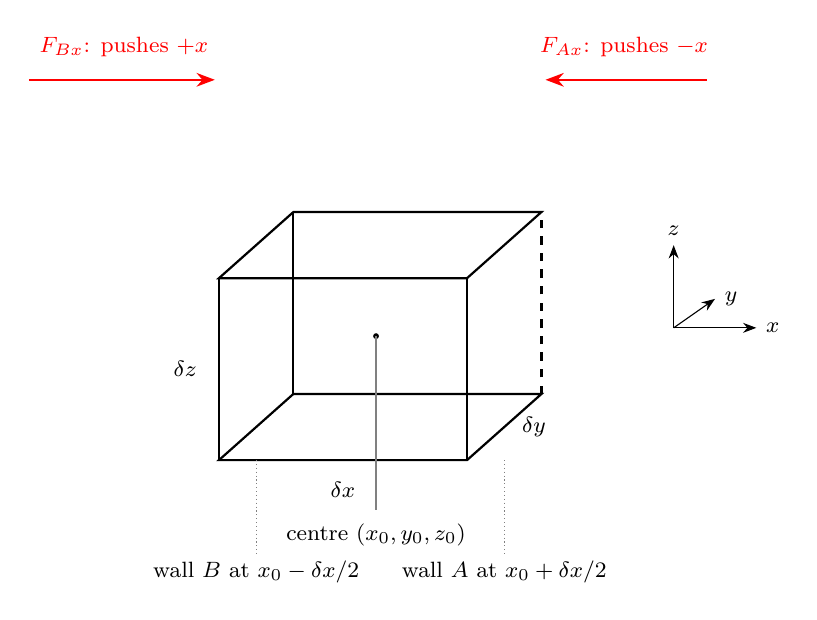
\begin{tikzpicture}[scale=1.05, >=Stealth]
% Box (simple parallelepiped in 2D projection)
\coordinate (A1) at (0,0);
\coordinate (A2) at (3,0);
\coordinate (A3) at (3.9,0.8);
\coordinate (A4) at (0.9,0.8);
\coordinate (B1) at (0,2.2);
\coordinate (B2) at (3,2.2);
\coordinate (B3) at (3.9,3.0);
\coordinate (B4) at (0.9,3.0);
\draw[thick] (A1)--(A2)--(A3)--(A4)--cycle;
\draw[thick] (B1)--(B2)--(B3)--(B4)--cycle;
\draw[thick] (A1)--(B1); \draw[thick] (A2)--(B2); \draw[thick,dashed] (A3)--(B3); \draw[thick] (A4)--(B4);
% Centre point, label placed well below the box
\fill (1.9,1.5) circle (1pt);
\draw[gray] (1.9,1.5) -- (1.9,-0.6);
\node[below] at (1.9,-0.65) {\footnotesize centre $(x_0,y_0,z_0)$};
% Wall labels placed just below the box, far from the coordinate label and from arrows
\node at (0.45,-1.35) {\footnotesize wall $B$ at $x_0-\delta x/2$};
\node at (3.45,-1.35) {\footnotesize wall $A$ at $x_0+\delta x/2$};
\draw[gray,densely dotted] (0.45,0) -- (0.45,-1.15);
\draw[gray,densely dotted] (3.45,0) -- (3.45,-1.15);
% Force arrows, well above the box, generously separated from every other label
\draw[->,thick,red] (5.9,4.6) -- (3.95,4.6);
\node[red] at (4.9,5.0) {\footnotesize $F_{Ax}$: pushes $-x$};
\draw[->,thick,red] (-2.3,4.6) -- (-0.05,4.6);
\node[red] at (-1.15,5.0) {\footnotesize $F_{Bx}$: pushes $+x$};
% axis triad, far right, clearly separated
\draw[->] (5.5,1.6) -- (6.5,1.6) node[right]{\footnotesize $x$};
\draw[->] (5.5,1.6) -- (5.5,2.6) node[above]{\footnotesize $z$};
\draw[->] (5.5,1.6) -- (6.0,1.95) node[right]{\footnotesize $y$};
% dimension labels
\node[below] at (1.5,-0.15) {\footnotesize $\delta x$};
\node[right] at (3.55,0.4){\footnotesize $\delta y$};
\node[left] at (-0.15,1.1){\footnotesize $\delta z$};
\end{tikzpicture}
\captionof{figure}{Fluid element used to derive the $x$-component of the pressure gradient force. Surrounding fluid pushes inward on every face; only the two faces normal to $x$ (wall $A$ at $x_0+\delta x/2$ and wall $B$ at $x_0-\delta x/2$) contribute to the net $x$-force, since pressure forces on the $y$- and $z$-faces have no $x$-component. $F_{Ax}$ (pushing $-x$, into the box from the $A$ side) and $F_{Bx}$ (pushing $+x$, into the box from the $B$ side) are drawn offset above the box purely for label clarity — both act \emph{on} the shaded volume, along $x$.}
\end{center}

Taylor-expand $p$ about the centre to first order. On wall $A$ (at $x_0+\delta x/2$), pressure $\approx p_0 + \dfrac{\partial p}{\partial x}\dfrac{\delta x}{2}$; this pushes the fluid element in the $-x$ direction (pressure pushes \emph{inward} on the volume), over area $\delta y\,\delta z$:
\begin{equation}
F_{Ax} = -\left(p_0+\frac{\partial p}{\partial x}\frac{\delta x}{2}\right)\delta y\,\delta z.
\end{equation}
On wall $B$ (at $x_0-\delta x/2$), pressure $\approx p_0 - \dfrac{\partial p}{\partial x}\dfrac{\delta x}{2}$, pushing in the $+x$ direction:
\begin{equation}
F_{Bx} = +\left(p_0-\frac{\partial p}{\partial x}\frac{\delta x}{2}\right)\delta y\,\delta z.
\end{equation}
Sum:
\begin{equation}
F_x = F_{Ax}+F_{Bx} = -\frac{\partial p}{\partial x}\,\delta x\,\delta y\,\delta z.
\end{equation}
The higher-order Taylor terms vanish as $\delta x,\delta y,\delta z\to0$; this is why the net force is proportional to the \emph{gradient} of $p$ (not $p$ itself — a spatially uniform pressure exerts zero net force, since the pushes on opposite faces exactly cancel). Divide by the mass $m=\rho\,\delta x\,\delta y\,\delta z$ to get the force \emph{per unit mass}:
\begin{equation}
\frac{F_x}{m} = -\frac{1}{\rho}\frac{\partial p}{\partial x}.
\end{equation}
Identical reasoning for the $y$- and $z$-faces gives $F_y/m = -\rho^{-1}\partial p/\partial y$ and $F_z/m=-\rho^{-1}\partial p/\partial z$ (this $z$-component, combined with gravity, reproduces the hydrostatic equation \eqref{eq:hydrostatic} as the special case of \emph{zero net vertical force}). Collecting all three components as a vector:
\begin{equation}
\boxed{\frac{\mathbf F_{\rm pg}}{m} = -\frac{1}{\rho}\nabla p}
\label{eq:pgf}
\end{equation}
the \textbf{pressure gradient force per unit mass}. It points from high toward low pressure, with magnitude proportional to how rapidly $p$ changes in space, and is completely independent of the pressure's absolute value.

\subsection{Gravitational force}
Newton's law of gravitation: two point masses $M,m$ separated by $\mathbf r$ (directed from $M$ toward $m$, $r=|\mathbf r|$) attract with force on $m$:
\begin{equation}
\mathbf F_g = -\frac{GMm}{r^2}\hat{\mathbf r}, \qquad \hat{\mathbf r}=\mathbf r/r.
\end{equation}
For finite bodies this still holds with $r$ = distance between centres of mass (a consequence of the shell theorem for spherically symmetric bodies, itself provable by integrating Newton's law over a spherical shell — standard result, not re-derived here). For the atmosphere ($m$ = a unit atmospheric mass element, $M$ = Earth's mass), the force \emph{per unit mass} is
\begin{equation}
\mathbf g^{*} \equiv \frac{\mathbf F_g}{m} = -\frac{GM}{r^2}\hat{\mathbf r}.
\label{eq:gravity}
\end{equation}
$\mathbf g^*$ is the \emph{true} gravitational acceleration; the \emph{effective} gravity $\mathbf g$ used in \S\ref{sec:hydrostatic} additionally includes a small centrifugal correction due to Earth's rotation (not derived in the source material; flagged here as the reason $g$ in Table 2 varies slightly with latitude as well as height, beyond the pure $1/r^2$ falloff of $\mathbf g^*$).

\subsection{Scales of atmospheric motion}
The pressure gradient force (and the other forces: Coriolis, friction, gravity) dominate different types of motion depending on horizontal scale:

\begin{table}[h!]
\centering
\begin{tabular}{@{}lc@{}}
\toprule
Type of motion & Horizontal scale (m) \\
\midrule
Molecular mean free path & $10^{-7}$ \\
Minute turbulent eddies & $10^{-2}$--$10^{-1}$ \\
Small eddies & $10^{-1}$--$1$ \\
Dust devils & $1$--$10$ \\
Gusts & $10$--$10^{2}$ \\
Tornadoes & $10^{2}$ \\
Cumulonimbus clouds & $10^{3}$ \\
Fronts, squall lines & $10^{4}$--$10^{5}$ \\
Hurricanes & $10^{5}$ \\
Synoptic cyclones & $10^{6}$ \\
Planetary waves & $10^{7}$ \\
\bottomrule
\end{tabular}
\caption{Characteristic horizontal scales of atmospheric motions (Holton). Rotational (Coriolis) effects become dynamically important only for the larger scales in this table ($\gtrsim10^5$--$10^6$ m), which is why small-scale phenomena (dust devils, tornadoes) are governed essentially by pressure gradient force balanced against centrifugal/frictional effects, without rotation of the Earth playing a leading role.}
\end{table}

% =====================================================================
\section{The Global Radiative Energy Balance}
\label{sec:radbalance}

\subsection{Blackbody radiation: Stefan--Boltzmann and Wien laws (empirical inputs)}
Two empirical facts about thermal (blackbody) radiation are used without re-derivation (their derivation requires quantum statistical mechanics, out of scope):
\begin{align}
\textbf{Stefan--Boltzmann law:}\quad & F = \sigma T^4, \qquad \sigma = 5.67\times10^{-8}\ \si{\watt\per\square\m\per\kelvin\tothe{4}} \label{eq:SB}\\
\textbf{Wien's displacement law:}\quad & \lambda_m T = \text{const} \label{eq:wien}
\end{align}
where $F$ is the total (wavelength-integrated) power radiated per unit area by an ideal blackbody at temperature $T$, and $\lambda_m$ is the wavelength at which its emission spectrum peaks.

\begin{worked}[Where does the terrestrial spectrum peak?]
Sun: $T_{\rm sun}\approx6000$ K, peak $\lambda_m\approx0.6\ \mu$m (visible). Earth's emission temperature $T_e=255$ K (derived below). By Wien's law \eqref{eq:wien}, $\lambda_m^{\rm Earth}/\lambda_m^{\rm sun} = T_{\rm sun}/T_e$, so
\[
\lambda_m^{\rm Earth} = 0.6\ \mu\text{m}\times\frac{6000}{255} \approx 14\ \mu\text{m} \quad(\text{thermal infrared}).
\]
Because solar emission peaks in the visible ($\sim$0.5 $\mu$m) and terrestrial emission peaks in the thermal IR ($\sim$14 $\mu$m) — a factor of $\sim$20 apart — the two spectra barely overlap. This separation is what allows ``shortwave'' (solar) and ``longwave'' (terrestrial) radiation to be treated as two essentially independent radiative streams, each with its own characteristic interaction with atmospheric gases (\S\ref{sec:absorption}).
\end{worked}

\subsection{Planetary emission temperature}
\label{sec:Te}

The Sun radiates total power $Q=3.87\times10^{26}$ W (constant on the timescale of interest). At the Earth's orbital distance $r$, this power is spread over a sphere of area $4\pi r^2$, giving the \textbf{solar constant}
\begin{equation}
S_0 = \frac{Q}{4\pi r^2}.
\end{equation}
For Earth ($r=150\times10^9$ m), $S_0=1367\ \si{\watt\per\square\m}$.

The Earth presents a \emph{disc} of cross-sectional area $\pi a^2$ ($a$ = Earth's radius) to the incoming parallel solar beam, so the total power intercepted is $S_0\pi a^2$. A fraction $\alpha_p$ (the \textbf{planetary albedo}, $\alpha_p\approx0.30$ for Earth) is reflected directly back to space without being absorbed; the absorbed power is
\begin{equation}
P_{\rm abs} = (1-\alpha_p)S_0\pi a^2.
\label{eq:Pabs}
\end{equation}

In energy balance (steady state), the Earth must radiate this same power back to space. Modelling the (spinning, quickly-rotating) Earth as an isothermal blackbody sphere of \emph{effective} temperature $T_e$ radiating over its \emph{full} surface area $4\pi a^2$ (a sphere, not just the sunlit disc — this is what distinguishes the emitting geometry from the absorbing geometry and is the origin of the factor of 4 below), Stefan--Boltzmann \eqref{eq:SB} gives
\begin{equation}
P_{\rm emit} = 4\pi a^2\,\sigma T_e^4.
\label{eq:Pemit}
\end{equation}
Equate \eqref{eq:Pabs} and \eqref{eq:Pemit} (steady-state energy balance) and cancel $\pi a^2$ (note $a$ itself cancels completely — $T_e$ does not depend on planet size):
\begin{equation}
4\sigma T_e^4 = (1-\alpha_p)S_0 \quad\Longrightarrow\quad \boxed{T_e = \left[\frac{S_0(1-\alpha_p)}{4\sigma}\right]^{1/4}}.
\label{eq:Te}
\end{equation}
Numerically, for Earth: $T_e = \left[\dfrac{1367\times0.70}{4\times5.67\times10^{-8}}\right]^{1/4} = 255\ \text{K}$.

\begin{intuition}[Why the factor of 4?]
The factor 4 is purely geometric: $4\pi a^2$ (sphere, emits in all directions, all the time, day \emph{and} night side) versus $\pi a^2$ (disc, only the cross-section facing the sun intercepts sunlight). Equivalently: $S_0/4$ is the solar flux \emph{averaged over the entire spherical surface} of the Earth (accounting for the fact that only half the sphere faces the sun at any instant, and even the sunlit half receives flux at an oblique angle except at the sub-solar point — averaging $\cos\theta$ over a hemisphere and dividing by the full sphere area reproduces exactly the factor of $1/4$).
\end{intuition}

Crucially, $T_e=255$ K is \emph{not} the surface temperature — it is the temperature the planet \emph{appears} to have when viewed from space (i.e.\ the temperature of the effective emitting level), which by the greenhouse effect (\S\ref{sec:greenhouse}) differs substantially from the actual surface temperature $T_s=288\ \text{K}$.

\begin{table}[h!]
\centering
\begin{tabular}{@{}lccccccc@{}}
\toprule
Planet & $r$ ($10^9$m) & $S_0$ (W/m$^2$) & $\alpha_p$ & $T_e$ (K) & $T_m$ (K, measured) & $T_s$ (K) \\
\midrule
Venus & 108 & 2632 & 0.77 & 227 & 230 & 760 \\
Earth & 150 & 1367 & 0.30 & 255 & 250 & 288 \\
Mars & 228 & 589 & 0.24 & 211 & 220 & 230 \\
Jupiter & 780 & 51 & 0.51 & 103 & 130 & 134 \\
\bottomrule
\end{tabular}
\caption{Emission temperature \eqref{eq:Te} vs.\ measured emission temperature $T_m$ and actual surface temperature $T_s$. Agreement between $T_e$ and $T_m$ is excellent for Venus, Earth, Mars — confirming \eqref{eq:Te} as a good description of \emph{radiative} balance at the top of atmosphere. Jupiter is the outlier because roughly half its emitted energy comes from internal gravitational contraction, not reprocessed sunlight, violating the assumption that all emitted power originates from absorbed solar power.}
\end{table}

\subsection{Albedo}
$\alpha_p$ (planetary, i.e.\ top-of-atmosphere average) differs from \emph{surface} albedo, which varies hugely by surface type:

\begin{table}[h!]
\centering
\begin{tabular}{@{}lc@{}}
\toprule
Surface & Albedo (\%) \\
\midrule
Ocean & 2--10 \\
Forest & 6--18 \\
Grass/grassland & 7--25 \\
Soil & 10--20 \\
Desert (sand) & 35--45 \\
Cloud (thin/thick) & 30 / 60--70 \\
Old snow & 40--60 \\
Fresh snow & 75--95 \\
\bottomrule
\end{tabular}
\caption{Surface albedo by type. Clouds and snow/ice dominate the \emph{planetary} albedo budget because of both their high individual albedo and their large areal coverage — this is the physical basis of the ice-albedo feedback (\S\ref{sec:feedback}).}
\end{table}

\subsection{The atmospheric absorption spectrum}
\label{sec:absorption}
Plotting fractional absorption vs.\ wavelength for a vertical path through the atmosphere reveals:
\begin{itemize}[leftmargin=1.4em]
\item Near-total transparency in the visible (where solar flux peaks) — sunlight reaches the surface largely unimpeded.
\item Strong, broadband opacity in the UV (ozone absorption — protects the biosphere, and is why stratospheric ozone heating occurs).
\item Highly wavelength-selective (``patchy'') opacity across the IR (where terrestrial flux peaks): nearly opaque at some wavelengths (e.g.\ the CO$_2$ 15 $\mu$m band, H$_2$O bands), nearly transparent in narrow ``atmospheric windows'' (e.g.\ $\sim$10--12 $\mu$m).
\item N$_2$ contributes essentially no absorption anywhere in this range; O$_2$ absorbs only in the far UV and weakly in the near-IR. The dominant absorbers, despite being trace constituents, are the triatomic molecules H$_2$O, CO$_2$, O$_3$ (and others), precisely because of their vibrational/rotational mode structure (see Intuition box in \S\ref{sec:composition}).
\end{itemize}
This selective, patchy IR opacity is exactly what makes the ``single infinitely-opaque slab'' idealization of \S\ref{sec:greenhouse} only a first approximation, motivating the ``leaky greenhouse'' refinement.

% =====================================================================
\section{Greenhouse Models: From Zero-Dimensional Balance to a Radiating Atmosphere}
\label{sec:greenhouse}

All models below share the same logical structure: write down zero-net-flux (energy balance) conditions at each interface (top of atmosphere, surface, and — if present — each internal atmospheric layer), then solve the resulting linear system for temperatures. All use the \emph{planar} (flat-slab) approximation, replacing the full spherical geometry by using the disc-averaged flux $S_0(1-\alpha_p)/4$ (already incorporating the same factor of 4 derived in \S\ref{sec:Te}) as the ``incoming solar flux per unit area'' striking a flat surface.

\subsection{Model 1: single opaque atmospheric layer}
\label{sec:model1}

\textbf{Assumptions}: (i) the atmosphere (single layer, temperature $T_a$) is completely transparent to solar (shortwave) radiation; (ii) it is completely opaque to terrestrial (longwave/IR) radiation — it absorbs \emph{all} upwelling IR from the surface.

\begin{center}
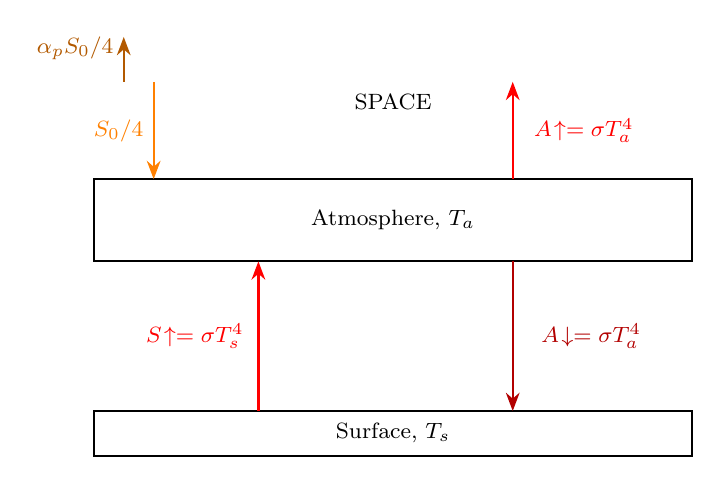
\begin{tikzpicture}[scale=0.95,>=Stealth]
\draw[thick] (0,0) rectangle (8,1.1); % atmosphere band
\node at (4,0.55) {\footnotesize Atmosphere, $T_a$};
\draw[thick] (0,-2.6) rectangle (8,-2.0); % surface band (thin), moved further down
\node at (4,-2.3) {\footnotesize Surface, $T_s$};
\node[above] at (4,1.9) {\footnotesize SPACE};
% incoming solar
\draw[->,thick,orange] (0.8,2.4) -- (0.8,1.1) node[midway,left,orange]{\footnotesize $S_0/4$};
\draw[->,thick,orange!70!black] (0.4,2.4) -- (0.4,3.0) node[near end,left]{\footnotesize $\alpha_p S_0/4$};
% up from ground -- own column, label to the LEFT
\draw[->,thick,red] (2.2,-2.0) -- (2.2,0);
\node[red] at (1.35,-1.0) {\footnotesize $S\!\uparrow=\sigma T_s^4$};
% down from atmos to ground -- own column, well separated, label to the RIGHT
\draw[->,thick,red!70!black] (5.6,0) -- (5.6,-2.0);
\node[red!70!black] at (6.65,-1.0) {\footnotesize $A\!\downarrow=\sigma T_a^4$};
% up from atmos to space
\draw[->,thick,red] (5.6,1.1) -- (5.6,2.4);
\node[red] at (6.55,1.75) {\footnotesize $A\!\uparrow=\sigma T_a^4$};
\end{tikzpicture}
\captionof{figure}{Model 1: single fully-opaque atmospheric slab. All upwelling IR from the ground ($S\uparrow$) is absorbed by the atmosphere layer and re-emitted equally up ($A\uparrow$) and down ($A\downarrow$), each $=\sigma T_a^4$ by Stefan--Boltzmann applied to the (isothermal) layer.}
\end{center}

\textbf{Top-of-atmosphere balance} (absorbed solar = emitted-to-space IR, since the layer is opaque, only $A\uparrow$ escapes):
\begin{equation}
\sigma T_a^4 = \frac{1}{4}(1-\alpha_p)S_0 = \sigma T_e^4 \quad\Longrightarrow\quad T_a = T_e.
\label{eq:model1_toa}
\end{equation}
(Sensible: the layer that is actually radiating to space \emph{is}, by the definition of \S\ref{sec:Te}, at the emission temperature.)

\textbf{Surface balance} (zero net flux at ground: absorbed solar + downwelling atmospheric IR = upwelling surface IR):
\begin{equation}
\sigma T_s^4 = \frac{1}{4}(1-\alpha_p)S_0 + \sigma T_a^4 = \sigma T_e^4+\sigma T_e^4 = 2\sigma T_e^4
\end{equation}
using \eqref{eq:model1_toa}. Hence
\begin{equation}
\boxed{T_s = 2^{1/4}T_e \approx 1.19\,T_e}.
\label{eq:model1_result}
\end{equation}
Numerically: $T_s = 2^{1/4}\times255 = 303$ K — an \emph{overestimate} of the true $T_s=288$ K, because assuming total IR opacity overstates the greenhouse effect (see \S\ref{sec:absorption}: real absorption is incomplete/patchy).

\subsection{Model 2: the ``leaky'' greenhouse}
\label{sec:leaky}

Relax assumption (ii): let the atmosphere have IR \textbf{absorptivity} $\epsilon\in[0,1]$, i.e.\ it absorbs only a fraction $\epsilon$ of the upwelling surface IR and \emph{transmits} the remaining fraction $(1-\epsilon)$ straight through to space.

\begin{center}
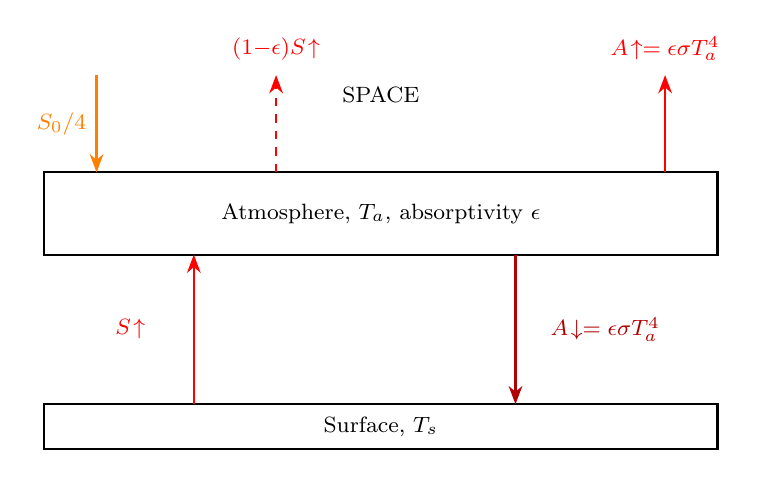
\begin{tikzpicture}[scale=0.95,>=Stealth]
\draw[thick] (0,0) rectangle (9,1.1);
\node at (4.5,0.55) {\footnotesize Atmosphere, $T_a$, absorptivity $\epsilon$};
\draw[thick] (0,-2.6) rectangle (9,-2.0);
\node at (4.5,-2.3) {\footnotesize Surface, $T_s$};
\node[above] at (4.5,1.9) {\footnotesize SPACE};
% incoming solar, far left
\draw[->,thick,orange] (0.7,2.4) -- (0.7,1.1) node[midway,left,orange]{\footnotesize $S_0/4$};
% S-up from ground, own column
\draw[->,thick,red] (2.0,-2.0) -- (2.0,0);
\node[red] at (1.15,-1.0) {\footnotesize $S\!\uparrow$};
% dashed direct transmission, its OWN column, offset from S-up
\draw[->,thick,red,dashed] (3.1,1.1) -- (3.1,2.4);
\node[red] at (3.1,2.75) {\footnotesize $(1{-}\epsilon)S\!\uparrow$};
% A-down, own column to the right, label to the right
\draw[->,thick,red!70!black] (6.3,0) -- (6.3,-2.0);
\node[red!70!black] at (7.5,-1.0) {\footnotesize $A\!\downarrow=\epsilon\sigma T_a^4$};
% A-up to space, far right column
\draw[->,thick,red] (8.3,1.1) -- (8.3,2.4);
\node[red] at (8.3,2.75) {\footnotesize $A\!\uparrow=\epsilon\sigma T_a^4$};
\end{tikzpicture}
\captionof{figure}{Leaky greenhouse: a fraction $(1-\epsilon)$ of surface IR ($S\uparrow$) passes straight through the atmosphere to space (dashed arrow) without interacting; only the absorbed fraction $\epsilon S\uparrow$ is re-emitted by the layer, split equally up and down as $A\uparrow=A\downarrow=\epsilon\sigma T_a^4$ (Kirchhoff's law: emissivity = absorptivity, applied below).}
\end{center}

\textbf{TOA balance}: absorbed solar = (directly transmitted surface IR) + (atmosphere's own emission to space):
\begin{equation}
\frac{1}{4}(1-\alpha_p)S_0 = A\uparrow + (1-\epsilon)S\uparrow.
\label{eq:leaky_toa}
\end{equation}
\textbf{Surface balance}: absorbed solar + downwelling atmospheric IR = upwelling surface IR:
\begin{equation}
\frac{1}{4}(1-\alpha_p)S_0 + A\downarrow = S\uparrow.
\label{eq:leaky_sfc}
\end{equation}
\textbf{Kirchhoff's law} (emissivity = absorptivity for a body in local thermodynamic equilibrium — stated here as an empirical/thermodynamic input): since the layer absorbs a fraction $\epsilon$ of incident IR, it also emits with efficiency $\epsilon$ relative to a full blackbody at $T_a$, in \emph{each} direction:
\begin{equation}
A\uparrow = A\downarrow = \epsilon\,\sigma T_a^4.
\label{eq:kirchhoff}
\end{equation}
Since $A\uparrow=A\downarrow$, subtract \eqref{eq:leaky_toa} from \eqref{eq:leaky_sfc}... more directly, add \eqref{eq:leaky_toa} and \eqref{eq:leaky_sfc} is not the efficient route; instead substitute $A\downarrow=A\uparrow$ (from \eqref{eq:kirchhoff}) into \eqref{eq:leaky_sfc}, and note \eqref{eq:leaky_toa} gives $A\uparrow = \tfrac14(1-\alpha_p)S_0 - (1-\epsilon)S\uparrow = \sigma T_e^4-(1-\epsilon)S\uparrow$. Insert into \eqref{eq:leaky_sfc}:
\begin{equation}
\sigma T_e^4 + \left[\sigma T_e^4 - (1-\epsilon)S\uparrow\right] = S\uparrow
\ \Longrightarrow\ 2\sigma T_e^4 = S\uparrow\left[1+(1-\epsilon)\right] = (2-\epsilon)S\uparrow.
\end{equation}
With $S\uparrow=\sigma T_s^4$:
\begin{equation}
\boxed{T_s = \left(\frac{2}{2-\epsilon}\right)^{1/4}T_e}.
\label{eq:leaky_result}
\end{equation}
\textbf{Limits}: $\epsilon\to0$ (perfectly transparent atmosphere, no greenhouse effect) $\Rightarrow T_s\to T_e$; $\epsilon\to1$ (fully opaque) $\Rightarrow T_s\to2^{1/4}T_e$, recovering Model 1 \eqref{eq:model1_result} exactly, as it must. For any $0<\epsilon<1$: $T_e<T_s<2^{1/4}T_e$ — \emph{partial} opacity gives a \emph{partial} greenhouse enhancement, interpolating smoothly between the two limits.

The atmospheric-layer temperature follows from combining \eqref{eq:kirchhoff}, \eqref{eq:leaky_toa}--\eqref{eq:leaky_sfc}:
\begin{equation}
T_a = \left(\frac{1}{2-\epsilon}\right)^{1/4}T_e = \left(\frac{1}{2}\right)^{1/4}T_s,
\end{equation}
so the atmosphere is \emph{always} cooler than the surface for $\epsilon<1$ ($T_a<T_e\le$ well, more precisely $T_a<T_s$ always, and $T_a<T_e$ strictly for $\epsilon<1$).

\subsection{Model 3: multi-layer (``more opaque'') greenhouse}
\label{sec:multilayer}

To go beyond a single slab, stack $N$ layers, each individually totally IR-opaque (absorbs everything incident on it, re-emits according to its own temperature, up and down). With $N=2$ (layers A above B, B just above the ground):

\begin{center}
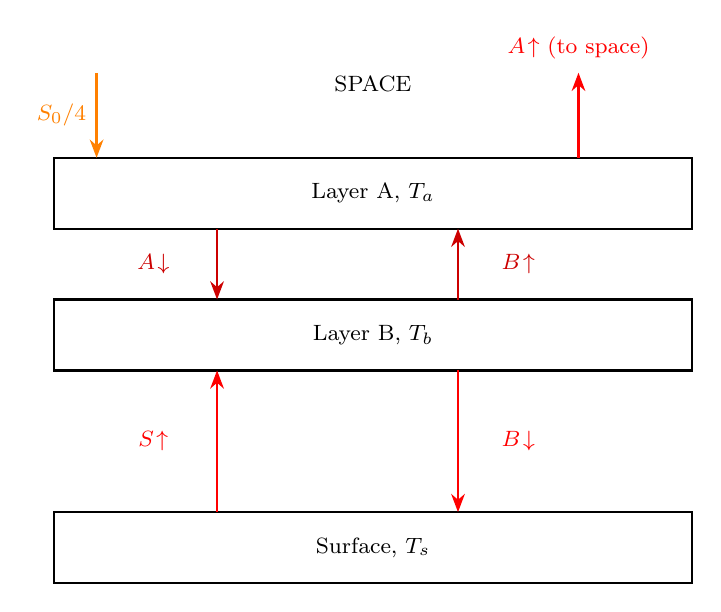
\begin{tikzpicture}[scale=0.9,>=Stealth]
\draw[thick] (0,3.4) rectangle (9,4.4); \node at (4.5,3.9) {\footnotesize Layer A, $T_a$};
\draw[thick] (0,1.4) rectangle (9,2.4); \node at (4.5,1.9) {\footnotesize Layer B, $T_b$};
\draw[thick] (0,-1.6) rectangle (9,-0.6); \node at (4.5,-1.1) {\footnotesize Surface, $T_s$};
\node[above] at (4.5,5.2) {\footnotesize SPACE};
\draw[->,thick,orange] (0.6,5.6) -- (0.6,4.4) node[midway,left,orange]{\footnotesize $S_0/4$};
\draw[->,thick,red] (7.4,4.4) -- (7.4,5.6);
\node[red] at (7.4,5.95) {\footnotesize $A\!\uparrow$ (to space)};
\draw[->,thick,red!80!black] (5.7,2.4) -- (5.7,3.4);
\node[red!80!black] at (6.55,2.9) {\footnotesize $B\!\uparrow$};
\draw[->,thick,red!80!black] (2.3,3.4) -- (2.3,2.4);
\node[red!80!black] at (1.4,2.9) {\footnotesize $A\!\downarrow$};
\draw[->,thick,red] (2.3,-0.6) -- (2.3,1.4);
\node[red] at (1.4,0.4) {\footnotesize $S\!\uparrow$};
\draw[->,thick,red] (5.7,1.4) -- (5.7,-0.6);
\node[red] at (6.55,0.4) {\footnotesize $B\!\downarrow$};
\end{tikzpicture}
\captionof{figure}{Two-layer opaque greenhouse: each layer fully absorbs whatever IR is incident on it from below or above and re-emits at its own temperature, up and down. Because the ground no longer directly ``sees'' space (layer A does), more layers systematically raise $T_s$ relative to $T_e$ compared to the single-layer model.}
\end{center}

Applying zero-net-flux at each of the three interfaces (space/A, A/B, B/surface) and Kirchhoff's law at each layer gives (by an argument fully analogous to \S\ref{sec:model1}, extended by induction) $T_a=T_e$ (topmost layer, the one that ``sees'' space, is at $T_e$, exactly as in Model 1), and successively warmer layers beneath. In general, for $N$ stacked, fully opaque, isothermal layers, one can show $\sigma T_s^4 = (N+1)\sigma T_e^4$, i.e.\ $T_s=(N+1)^{1/4}T_e$ — each additional fully-opaque layer further raises the surface temperature (though with diminishing fractional effect, since $T_s\propto (N+1)^{1/4}$, a slowly-growing function of $N$).

\textbf{The radiative equilibrium profile and its discontinuity.} Taking the continuum limit ($N\to\infty$, each layer infinitesimally thin, with realistic vertical distributions of H$_2$O, CO$_2$, O$_3$ replacing the crude ``fully opaque'' assumption) yields the \textbf{radiative equilibrium temperature profile}: the temperature structure that \emph{would} exist if vertical heat transport occurred \emph{purely} by radiative transfer (no convection, no fluid motion). This calculated profile has a striking feature: a large temperature \textbf{discontinuity right at the surface} — the radiative-equilibrium ground temperature is far warmer than the air immediately above it. This is \emph{not} observed in the real atmosphere (\S\ref{sec:radconv}).

\begin{intuition}[Why the radiative discontinuity arises, and why it's unphysical]
In the multilayer models above, \emph{most solar radiation reaches and is absorbed directly at the surface} (the atmosphere is comparatively transparent to shortwave, per \S\ref{sec:absorption}), while the atmosphere absorbs and re-emits IR layer by layer. A surface heated directly by the (large) solar flux, radiating IR only through the (comparatively poor) bucket-brigade of layer-by-layer IR transfer, ends up radiatively \emph{much} warmer than the air just above it. But a fluid cannot sustain an infinitely sharp temperature discontinuity at its lower boundary with warm, buoyant air sitting directly beneath cooler air: this configuration is \textbf{unstable to convection}. The real atmosphere responds by convectively overturning, mixing heat upward mechanically and erasing the discontinuity — which is exactly the physics developed in \S\ref{sec:radconv}.
\end{intuition}

\subsection{Climate sensitivity and feedbacks}
\label{sec:feedback}

Define \textbf{climate sensitivity} $\partial T_s/\partial Q$: the surface-temperature response to a small perturbation $\delta Q$ (units \si{\watt\per\square\m}) in the energy balance.

\textbf{Blackbody (Planck) feedback.} The dominant \emph{negative} feedback: a warmer planet radiates more, which opposes further warming. From $Q=\sigma T_e^4$ (treating $T_s$ and $T_e$ as differing by a fixed offset, so $\delta T_s = \delta T_e$), linearize:
\begin{equation}
\delta Q = 4\sigma T_e^3\,\delta T_s \quad\Longrightarrow\quad \left(\frac{\partial T_s}{\partial Q}\right)_{\rm BB} = \frac{1}{4\sigma T_e^3} = 0.26\ \si{\kelvin\per(\watt\per\square\m)}
\label{eq:BBfeedback}
\end{equation}
using $T_e=255$ K. This says a $1\ \si{\watt\per\square\m}$ increase in net forcing raises $T_s$ by only about a quarter of a degree, \emph{if this were the only feedback in play} — Planck feedback is the fundamental stabilizing mechanism of any radiating body.

\textbf{Water-vapour feedback (positive).} Saturation vapour pressure $e_s$ rises steeply with temperature (via the Clausius--Clapeyron relation, quoted here as $de_s/e_s = \beta\,dT$ with $\beta\approx0.067\ ^\circ\text{C}^{-1}$, i.e.\ roughly 7\% increase in saturation humidity per degree of warming — the precise molecular/thermodynamic derivation of Clausius--Clapeyron is outside the scope of the present excerpt). Since observed relative humidity stays roughly constant even as temperature varies seasonally, a warmer atmosphere \emph{actually holds} more water vapour — the dominant greenhouse gas — which further enhances the greenhouse effect and warms the surface further: a positive feedback that amplifies the bare Planck response. Combined Planck + water-vapour sensitivity is about
\begin{equation}
\left(\frac{\partial T_s}{\partial Q}\right)_{\rm BB+H_2O} \approx 0.5\ \si{\kelvin\per(\watt\per\square\m)},
\end{equation}
roughly double the blackbody-alone value \eqref{eq:BBfeedback}.

\textbf{Ice--albedo feedback (positive).} Ice/snow have very high albedo (Table 6) relative to open ocean or land. If warming melts ice, exposing darker underlying surface, absorbed solar radiation increases, causing further warming and further melt — a positive feedback, strongest at high latitudes where ice margins are most sensitive to temperature.

\textbf{Cloud feedback.} Clouds have high albedo and roughly double Earth's overall albedo from $\sim$15\% (clear-sky) to $\sim$30\% (all-sky), making cloud cover changes a major (and, in practice, highly uncertain in sign and magnitude) contributor to the total climate sensitivity — clouds can both cool (via albedo, reflecting sunlight) and warm (via greenhouse trapping of IR, especially high thin cirrus), and the net effect depends sensitively on cloud type, height, and optical thickness.

\begin{table}[h!]
\centering
\small
\begin{tabular}{@{}p{2.4cm}p{2.1cm}p{5.3cm}p{4cm}@{}}
\toprule
Feedback & Sign & Mechanism & Approx.\ sensitivity contribution \\
\midrule
Planck (blackbody) & Negative (stabilizing) & $\sigma T^4$ increases with $T$ & $0.26\ \si{\kelvin\per(\watt\per\square\m)}$ alone \\
Water vapour & Positive & warmer air holds more H$_2$O (greenhouse gas) & doubles Planck-alone value \\
Ice--albedo & Positive & melting exposes darker surface & largest at high latitude \\
Cloud & Uncertain sign & albedo (cooling) vs.\ IR trapping (warming) compete & largest source of model spread \\
\bottomrule
\end{tabular}
\caption{Summary of the principal climate feedbacks introduced by the simple greenhouse models.}
\end{table}

% =====================================================================
\section{Radiative--Convective Equilibrium}
\label{sec:radconv}

\subsection{Why pure radiative equilibrium fails near the surface}
Section \ref{sec:multilayer} showed that a purely radiative calculation predicts a surface temperature discontinuity: the ground is radiatively ``too hot'' relative to the air immediately above. Such a profile has temperature \emph{decreasing extremely rapidly} with height right near the ground — far faster than the \textbf{dry adiabatic lapse rate} $\Gamma_d$ (the rate at which a rising, unsaturated parcel cools simply due to expansion in lower pressure; a standard consequence of the first law of thermodynamics applied to a parcel undergoing adiabatic expansion, not re-derived in the present excerpt but used here as a known reference rate).

\begin{defbox}[Static stability criterion — used, not derived, here]
A layer is \emph{statically unstable} (will overturn convectively) if the actual environmental lapse rate exceeds the parcel's adiabatic cooling rate, i.e.\ if temperature falls with height \emph{faster} than $\Gamma_d$ (for unsaturated air) — equivalently, if a parcel nudged upward finds itself \emph{warmer} (hence more buoyant) than its new surroundings, accelerating further upward. The radiative-equilibrium discontinuity of \S\ref{sec:multilayer} is an extreme instance of exactly this instability, localized right at the surface.
\end{defbox}

\subsection{Convective adjustment}
When the radiative profile is unstable, convection spontaneously develops and transports heat upward \emph{mechanically} (via bulk motion of rising warm parcels and sinking cool parcels), not radiatively. This convective heat transport continues until the environmental temperature profile is adjusted back to (at most) marginal stability — i.e.\ until the lapse rate no longer exceeds the relevant adiabatic reference rate. The resulting steady state, combining radiative equilibrium \emph{above} the level convection reaches with a convectively-controlled profile \emph{below}, is called \textbf{radiative--convective equilibrium}.

\begin{center}
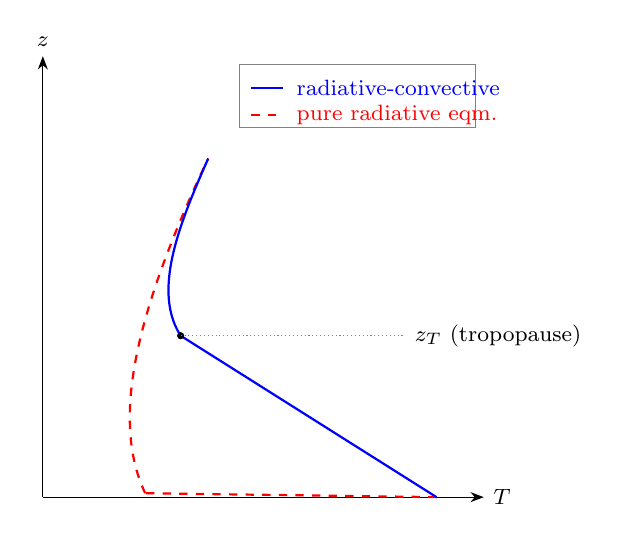
\begin{tikzpicture}[scale=1.0,>=Stealth]
\draw[->] (0,0) -- (0,5.6) node[above]{\footnotesize $z$};
\draw[->] (0,0) -- (5.6,0) node[right]{\footnotesize $T$};
% radiative equilibrium curve with big jump at surface
\draw[thick,red,dashed] (5.0,0) -- (1.3,0.05);
\draw[thick,red,dashed] (1.3,0.05) .. controls (0.85,1.0) and (1.2,2.4) .. (2.1,4.3);
% radiative-convective profile: straight adiabat near surface then merges
\draw[thick,blue] (5.0,0) -- (1.75,2.05);
\draw[thick,blue] (1.75,2.05) .. controls (1.4,2.6) and (1.7,3.4) .. (2.1,4.3);
\fill (1.75,2.05) circle(1.3pt);
\draw[gray,densely dotted] (1.75,2.05) -- (4.6,2.05);
\node[right] at (4.6,2.05) {\footnotesize $z_T$ (tropopause)};
% Legend box, well clear of both curves and axes, near the top
\draw[gray] (2.5,4.7) rectangle (5.5,5.5);
\draw[thick,blue] (2.65,5.2) -- (3.05,5.2);
\node[right,blue] at (3.1,5.2) {\footnotesize radiative-convective};
\draw[thick,red,dashed] (2.65,4.85) -- (3.05,4.85);
\node[right,red] at (3.1,4.85) {\footnotesize pure radiative eqm.};
\end{tikzpicture}
\captionof{figure}{Schematic radiative--convective equilibrium temperature profile (blue, solid) vs.\ the unphysical pure radiative-equilibrium profile (red, dashed) with its surface discontinuity. Below the level $z_T$ where convection reaches (in the tropics, roughly the tropopause), the profile follows a convectively-controlled (near-adiabatic) lapse rate; above $z_T$, radiative equilibrium is re-established and the two curves merge.}
\end{center}

\subsection{The tropical troposphere as a worked physical picture}
In the (moist, deep-convecting) tropics, observations show the troposphere is close to \emph{neutral for moist convection} essentially up to the tropopause height $z_T$ — i.e.\ convection is vigorous enough and frequent enough to keep the whole tropical troposphere near the moist-adiabatic reference profile. Physically:
\begin{itemize}[leftmargin=1.4em]
\item \textbf{Below $z_T$}: state is convectively determined (profile close to the moist adiabat).
\item \textbf{Above $z_T$}: convection cannot penetrate (stable stratosphere above), so the radiative-equilibrium state re-asserts itself.
\end{itemize}
This combination — convective control below, radiative control above, joined at the level convection reaches — is precisely the radiative-convective equilibrium structure sketched above, and constitutes a good first-order description of the observed tropical mean temperature profile.

Outgoing longwave radiation (OLR) provides an observational diagnostic that distinguishes these regimes:
\begin{itemize}[leftmargin=1.4em]
\item \textbf{Low OLR} regions: emission is coming from cold, high cloud tops (deep convective towers), consistent with radiation escaping from near the tropopause rather than the warm surface.
\item \textbf{High OLR} regions (e.g.\ subtropical deserts, cool dry ocean regions): skies are relatively clear and dry, so radiation escapes largely unimpeded from the warm surface itself.
\end{itemize}
Quantitatively, if the surface radiates as $\sigma T_s^4$ with $T_s\approx300$ K (tropics) but a deep convective cloud top radiates at $T_c\approx220$ K, the ratio of emitted flux is $(T_s/T_c)^4 \approx(300/220)^4\approx3.5$ — deep convective regions emit far less IR to space per unit area than clear, dry regions, which is exactly the OLR contrast used operationally (e.g.\ from satellites) to identify active convection.

\subsection{Requirements for convection}
Convection requires the surface to be warm \emph{relative to the air aloft}; two distinct routes achieve this:
\begin{enumerate}[leftmargin=1.4em]
\item \textbf{Surface heating} (e.g.\ solar heating of the ground) — drives the diurnal cycle of shallow/afternoon convection, strongest in summer and in the tropics.
\item \textbf{Upper-level cooling} (e.g.\ cold air advected aloft over a relatively warm surface) — the mechanism behind mid-latitude thunderstorms along cold fronts, where deep convection is typically \emph{intermittent} (episodic, tied to frontal passage) rather than the quasi-continuous deep convection of the tropics.
\end{enumerate}
In mid-latitudes, \emph{shallow} convection (visible as cumulus clouds) is common, but deep convection reaching the tropopause is intermittent; how the tropical radiative-convective temperature structure is communicated to higher latitudes is understood to be primarily through large-scale (synoptic) circulation systems transporting heat poleward, rather than through local convection at those latitudes.

% =====================================================================
\section{Consolidated Formula Reference}
\addcontentsline{toc}{section}{Consolidated Formula Reference}

\begin{table}[h!]
\centering
\small
\renewcommand{\arraystretch}{1.4}
\begin{tabular}{@{}p{5.6cm}p{9.6cm}@{}}
\toprule
\textbf{Relation} & \textbf{Formula} \\
\midrule
Ideal gas law (unit mass) & $p\alpha = RT$ \\
Universal gas law & $pV=nR^*T$, $R^*=8.3145\ \si{\joule\per\mol\per\kelvin}$ \\
Specific gas constant & $R=R^*/M$; $\Rd=287.0$, $\Rv=461.5\ \si{\joule\per\kg\per\kelvin}$ \\
Dalton's law & $p=\sum_i p_i$ \\
Virtual temperature & $T_v = T\big/\left[1-\tfrac{e}{p}(1-\varepsilon)\right]$, $\varepsilon=\Rd/\Rv=0.622$ \\
Hydrostatic equation & $\partial p/\partial z = -g\rho$ \\
Geopotential & $d\Phi = g\,dz = -\alpha\,dp$; $Z=\Phi/g_0$ \\
Hydrostatic + ideal gas & $d\Phi = -\Rd T_v\,d(\ln p)$ \\
Scale height & $H=\Rd T_v/g_0$; $p(Z)=p_1 e^{-(Z-Z_1)/H}$ \\
Hypsometric equation & $Z_2-Z_1 = \dfrac{\Rd\overline{T_v}}{g_0}\ln(p_1/p_2)$ \\
Pressure gradient force (per unit mass) & $\mathbf F_{\rm pg}/m = -\rho^{-1}\nabla p$ \\
Gravitational force (per unit mass) & $\mathbf g^*=-(GM/r^2)\hat{\mathbf r}$ \\
Stefan--Boltzmann law & $F=\sigma T^4$ \\
Wien's law & $\lambda_m T = \text{const}$ \\
Emission temperature & $T_e=\left[S_0(1-\alpha_p)/4\sigma\right]^{1/4}$ \\
Single-layer greenhouse & $T_s = 2^{1/4}T_e$ \\
Leaky greenhouse & $T_s = \left[2/(2-\epsilon)\right]^{1/4}T_e$ \\
Planck climate sensitivity & $\partial T_s/\partial Q = 1/(4\sigma T_e^3)$ \\
\bottomrule
\end{tabular}
\caption{All boxed/derived results collected for quick reference.}
\end{table}

\end{document}
